\documentclass[12pt]{article}
\usepackage{amsmath,amsfonts,times}
\usepackage{graphicx,color,tikz,pgfplots}
\usepackage[paperwidth=10.1cm,paperheight=8.1cm,lmargin=0in,rmargin=0in,tmargin=0.in,bmargin=0.in]{geometry}
\usepackage{bm}
\usetikzlibrary{arrows,shadings,shapes.arrows,decorations.pathreplacing,calc, positioning}
\usepgfplotslibrary{fillbetween}

\begin{document}
\centering
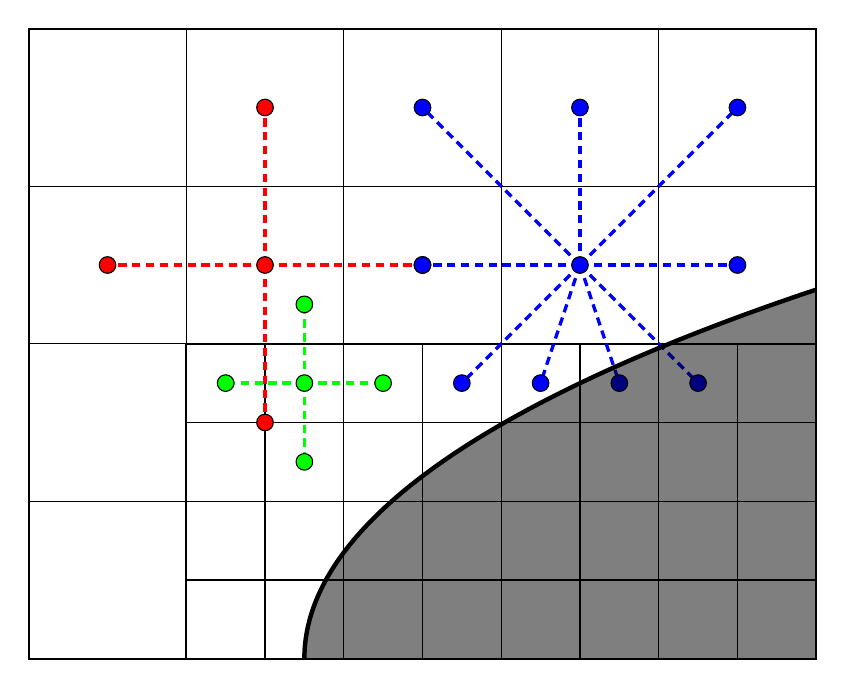
\begin{tikzpicture}[on grid]

  % Parent grid
  \draw[step=20mm, black, thin] (0,0) grid  (10,8); %defining grids
  \draw[black, thick] (0,0) rectangle (10,8); %marking borders

  % Refined grid
  \draw[step=10mm, black, thin] (2,0) grid  (10,4); %defining grids
  \draw[black, thick] (2,0) rectangle (10,4);%marking borders
  
  % Regular coarse stencil.
  \draw[very thick, red, densely dashed] (3,5) -- ++ ( 2, 0);
  \draw[very thick, red, densely dashed] (3,5) -- ++ (-2, 0);
  \draw[very thick, red, densely dashed] (3,5) -- ++ ( 0, 2);
  \draw[very thick, red, densely dashed] (3,5) -- ++ ( 0,-2);  
  \draw[black,fill=red] (3,7) circle (3pt);
  \draw[black,fill=red] (3,3) circle (3pt);
  \draw[black,fill=red] (1,5) circle (3pt);
  \draw[black,fill=red] (5,5) circle (3pt);
  \draw[black,fill=red] (3,5) circle (3pt);    

  % Regular fine stencil.
  \draw[very thick, green, densely dashed] (3.5,3.5) -- ++ ( 1, 0);
  \draw[very thick, green, densely dashed] (3.5,3.5) -- ++ (-1, 0);
  \draw[very thick, green, densely dashed] (3.5,3.5) -- ++ ( 0, 1);
  \draw[very thick, green, densely dashed] (3.5,3.5) -- ++ ( 0,-1);    
  \draw[black,fill=green] (3.5,3.5) circle (3pt);
  \draw[black,fill=green] (4.5,3.5) circle (3pt);
  \draw[black,fill=green] (2.5,3.5) circle (3pt);
  \draw[black,fill=green] (3.5,2.5) circle (3pt);
  \draw[black,fill=green] (3.5,4.5) circle (3pt);

  % Corrected coarse stencil
  \draw[very thick, blue, densely dashed] (7,5) --++ ( 2,0);
  \draw[very thick, blue, densely dashed] (7,5) --++ (-2,0);
  \draw[very thick, blue, densely dashed] (7,5) --++ ( 0,2);
  \draw[very thick, blue, densely dashed] (7,5) --++ ( 2,2);
  \draw[very thick, blue, densely dashed] (7,5) --++ (-2,2);
  \draw[very thick, blue, densely dashed] (7,5) --++ ( 0.5,-1.5);
  \draw[very thick, blue, densely dashed] (7,5) --++ (-0.5,-1.5);
  \draw[very thick, blue, densely dashed] (7,5) --++ (-1.5,-1.5);
  \draw[very thick, blue, densely dashed] (7,5) --++ ( 1.5,-1.5);    
  
  \draw[black,fill=blue] (5.0,5.0) circle (3pt);  
  \draw[black,fill=blue] (7.0,5.0) circle (3pt);
  \draw[black,fill=blue] (9.0,5.0) circle (3pt);
  \draw[black,fill=blue] (5.0,7.0) circle (3pt);  
  \draw[black,fill=blue] (7.0,7.0) circle (3pt);
  \draw[black,fill=blue] (9.0,7.0) circle (3pt);
  \draw[black,fill=blue] (5.5,3.5) circle (3pt);    
  \draw[black,fill=blue] (6.5,3.5) circle (3pt);  
  \draw[black,fill=blue] (7.5,3.5) circle (3pt);
  \draw[black,fill=blue] (8.5,3.5) circle (3pt);  

  %EB
  \clip(0,0) rectangle (10,8);  
  \draw[black, ultra thick, draw=black, fill=black, fill opacity=0.5] (53.5,0.0) ellipse (50cm and 9.5cm);



\end{tikzpicture}

\end{document} 
